% !TEX root = main.tex
% !TEX program = xelatex
\section{问题二的模型建立与求解}

\subsection{求解思路}

问题二要求每天0:00提前制定购电计划，但当天真实负载和光伏我们尚未可知。
同时我们还需考虑微网购电买多买少的问题。
如果电买少了，缺口需要按5倍电价紧急补购；买多了，如果无法使用或储存，仍需支付费用。
因此，问题二的核心是在\textbf{提前购电成本与紧急购电风险之间取得平衡}。

为此，我们决定依次比较三类方案：

\begin{enumerate}
    \item 利用历史同期数据预测负载和光伏；
    \item 引入岭回归和提升树，考察更复杂的预测方法能否降低实际费用；
    \item 最后在历史预测基础上加入误差准备，针对供需缺口被低估后可能产生的高价紧急购电进行防范；
\end{enumerate}

问题二的关键在于，问题的最终目标并不是使预测误差最小，而是使普通购电费用与紧急购电费用之和尽可能低。
同样大小的预测误差，如果发生在不同电价或不同储电状态下，其经济影响可能完全不同。

因此，我们最终选取\textbf{“历史分项预测—近期加权准备—跨日线性规划模型”}。
模型首先分别估计负载和光伏，再根据近期预测误差增加适量准备，随后利用线性规划制定普通购电计划。
白天普通订单保持不变，储能设备根据实际供需补充缺口或吸收余电，剩余缺口才通过紧急购电补足。


\subsection{供需预测与误差准备}

\subsubsection*{（1）负载与光伏预测}

探索性分析表明，负载具有明显的周重复特征，而光伏更适合参考近期水平。因此，负载取过去4个相同星期位置的平均，光伏取最近7天同一时刻的平均：

\begin{equation}
\widehat L_{d,k}
=
\frac{1}{4}\sum_{j=1}^{4}L_{d-7j,k},
\qquad
\widehat V_{d,k}
=
\frac{1}{7}\sum_{j=1}^{7}V_{d-j,k}.
\end{equation}

其中，$d$表示日期，$k$表示当天第$k$个10分钟时段。预测只使用当天0:00以前已经发生的数据，不提前读取当天真实值，也不使用问题三中的光伏预报。


\subsubsection*{（2）根据近期误差增加准备量}

仅使用平均预测，可能连续低估实际供需缺口，使电池过早降至储电下限。为此，定义历史净供需误差：

\begin{equation}
\varepsilon_{i,k}
=
\left[
(L_{i,k}-V_{i,k})
-
(\widehat L_{i,k}-\widehat V_{i,k})
\right]\Delta t .
\end{equation}

其中，$\varepsilon_{i,k}>0$表示实际供需缺口大于预测值，即原计划存在缺电风险。

本文取最近28天的误差，并按4小时分组。较新的误差给予更高权重，时间衰减参数取

\[
\beta=0.7.
\]

再取加权误差分布的$70\%$分位作为准备量，即

\[
\alpha=0.7.
\]

其中，$\beta$控制历史数据的新旧权重，$\alpha$控制准备程度。准备量加入预测净需求后，再交由后续调度模型统一安排，而不是在每个时段机械增加固定购电量。


\subsection{购电与储能优化模型}

每天0:00向前规划48小时，但只固定当天24小时的普通购电计划。这样既考虑当天费用，也避免模型在日末过度放空电池。

根据预测负载、预测光伏和准备量得到各时段预计净需求。模型设置外网充电量$x_t$、光伏充电量$y_t$、储能放电量$z_t$和内部储电量$S_t$。

普通购电量为

\begin{equation}
q_t=n_t-z_t+x_t.
\end{equation}

其含义是：预计负载缺口先由电池承担一部分，剩余部分由外网补足；当价格合适时，外网还可以额外购电给电池充电。

规划目标为最小化普通购电成本，并为48小时末剩余电量保留一定参考价值：

\begin{equation}
\min J
=
\sum_{t=1}^{288}p_tq_t-\nu S_{288}.
\end{equation}

其中，期末电量价值仅用于避免规划末端无意义地放空电池，不作为实际售电收入，也不从最终实际电费中扣除。

储能状态满足

\begin{equation}
S_t
=
S_{t-1}
+
0.9(x_t+y_t)
-
\frac{z_t}{0.9}.
\end{equation}

储电量必须满足

\begin{equation}
1200\leq S_t\leq10800.
\end{equation}

同时，储能设备充、放电功率均不超过5000 kW，因此每10分钟外侧最多充入或放出$833.33$ kWh。

问题二不再要求每天首尾储电量相等，而是将当天结束时的储电量直接作为下一天的初始储电量，实现跨日连续运行。

上述目标函数与约束均为线性关系，因此采用Python中SciPy的\texttt{linprog}接口调用HiGHS求解器进行求解。


\subsection{实际运行与紧急购电}

每天0:00确定普通购电计划后，白天不再修改普通订单，但电池可以根据实际负载和光伏动态充放电。

实际运行遵循以下原则：

\begin{itemize}
    \item 光伏优先直接供给负载；
    \item 普通购电不足时，电池在容量和功率允许范围内优先补充；
    \item 电池仍无法补足的部分才进行紧急购电；
    \item 若普通电和光伏有剩余，则在容量允许范围内给电池充电。
\end{itemize}

因此，第$d$天的实际购电费用为

\begin{equation}
C_d
=
\sum_{k=1}^{144}
\left(
p_kq_{d,k}
+
5p_ke_{d,k}
\right),
\end{equation}

其中，$e_{d,k}$为紧急购电量。当天结束后的储电量直接传递到下一天。

由此形成

\[
\text{零点制定计划}
\rightarrow
\text{白天实际运行}
\rightarrow
\text{电池吸收偏差}
\rightarrow
\text{必要时紧急补购}
\rightarrow
\text{库存传递至下一天}
\]

的连续调度过程。


\subsection{方案比较与求解结果}

本文比较了历史预测、岭回归、提升树以及加入不同误差准备方式的方案。评价标准不是单纯比较预测误差，而是比较实际产生的\textbf{普通购电费与紧急购电费之和}。

\begin{table}[H]
\centering
\caption{不同方案的实际购电费用}
\begin{tabular}{lccc}
\hline
方案 & 普通电费/万元 & 紧急电费/万元 & 总电费/万元 \\
\hline
历史预测，无准备 & 1218.58 & 374.70 & 1593.28 \\
岭回归，无准备 & 1210.27 & 446.88 & 1657.15 \\
提升树，无准备 & 1218.25 & 343.71 & 1561.96 \\
历史预测，等权准备 & 1295.99 & 107.05 & 1403.04 \\
历史预测，近期加权准备 & \textbf{1297.96} & \textbf{60.43} & \textbf{1358.38} \\
\hline
\end{tabular}
\end{table}

最终采用\textbf{历史预测 + 近期加权误差准备 + 线性规划调度}。

相比等权准备方案，近期加权虽然使普通电费增加约$1.97$万元，但紧急电费减少约$46.63$万元，总费用减少约$44.66$万元。说明其主要作用是通过提前做适量准备，减少高价紧急购电。

题目要求统计2025年2月1日至12月31日，共334天。最终总购电费用为

\[
\boxed{13583810.84\ \text{元}},
\]

其中普通购电费用为

\[
12979560.57\ \text{元},
\]

紧急购电费用为

\[
604250.27\ \text{元}.
\]


\subsubsection*{（1）月度费用分析}

图\ref{fig:q2_monthly_cost}给出了各月普通电费、紧急电费以及相对于等权准备方案的节省金额。

\begin{figure}[H]
    \centering
    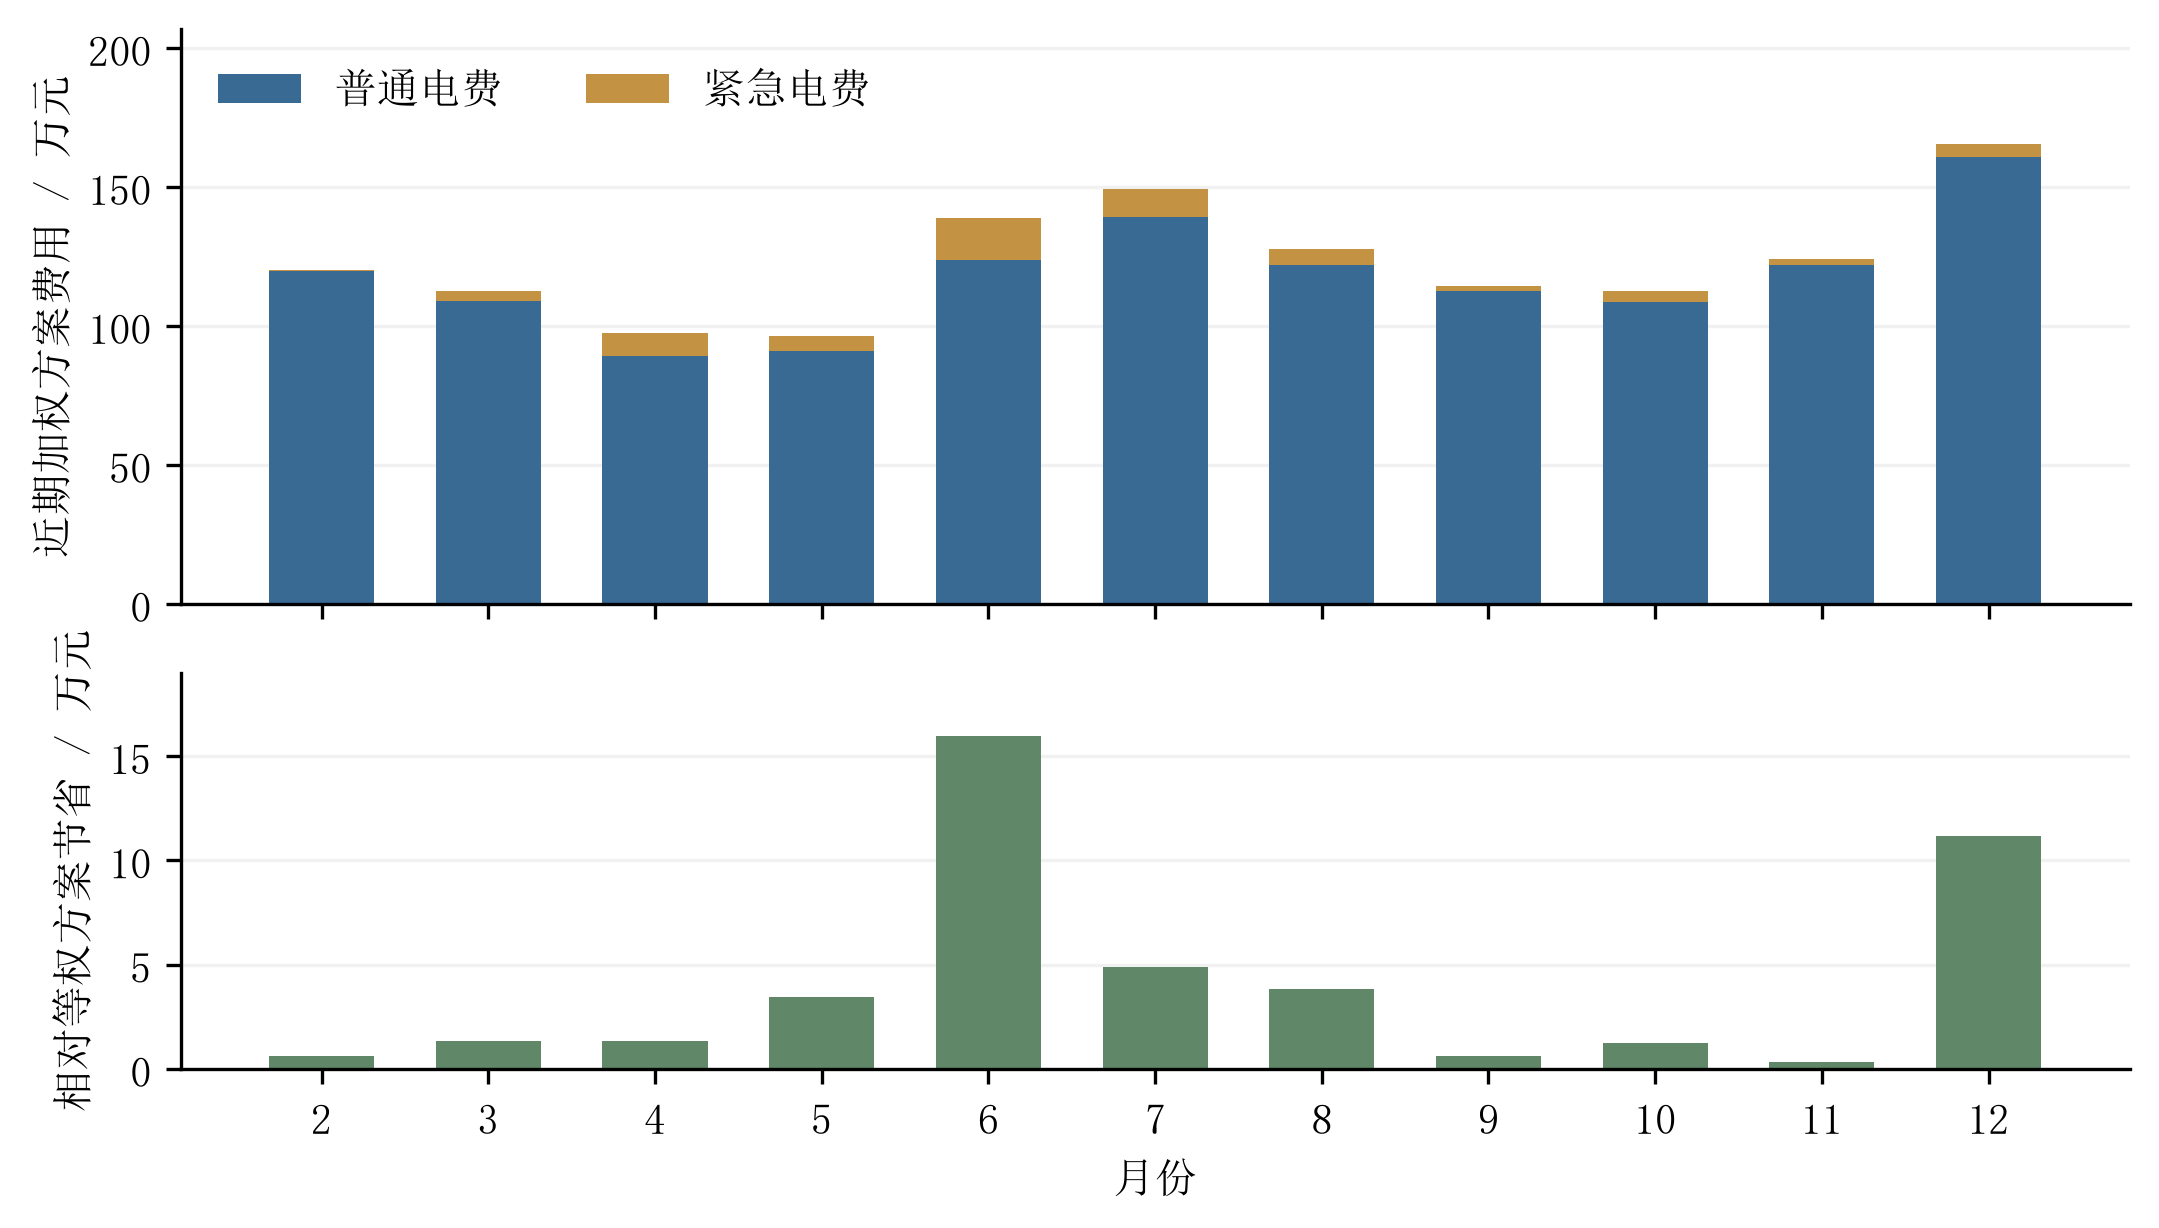
\includegraphics[width=0.95\textwidth]{fig/monthly_cost.png}
    \caption{近期加权准备方案的月度费用及相对等权准备的节省}
    \label{fig:q2_monthly_cost}
\end{figure}

由图\ref{fig:q2_monthly_cost}可见，各月份费用仍以普通购电为主，但紧急购电由于价格较高，对总费用影响明显。近期加权方案在11个月合计均取得节省，其中6月和12月贡献较大。

需要说明的是，该方案并非每天都更加便宜，而是在全年范围内通过减少高价紧急补购，使总费用进一步降低。


\subsubsection*{（2）指定日期运行分析}

题目指定日期的主要结果如下。

\begin{table}[H]
\centering
\caption{问题二：微网在指定日期的紧急购电量}
\begin{tabular}{|c|c|c|c|c|c|c|c|}
\hline
\multicolumn{2}{|c|}{2025.3.20} & \multicolumn{2}{c|}{2025.6.21} & \multicolumn{2}{c|}{2025.9.23} & \multicolumn{2}{c|}{2025.12.21} \\
\hline
时间段 & 购电量 & 时间段 & 购电量 & 时间段 & 购电量 & 时间段 & 购电量 \\
\hline
10:00--10:10 & 0.00 & 10:00--10:10 & 0.00 & 10:00--10:10 & 0.00 & 10:00--10:10 & 0.00 \\
\hline
12:00--12:10 & 610.16 & 12:00--12:10 & 0.00 & 12:00--12:10 & 484.48 & 12:00--12:10 & 943.63 \\
\hline
14:00--14:10 & 0.00 & 14:00--14:10 & 0.00 & 14:00--14:10 & 0.00 & 14:00--14:10 & 0.00 \\
\hline
16:00--16:10 & 434.90 & 16:00--16:10 & 116.65 & 16:00--16:10 & 453.86 & 16:00--16:10 & 798.03 \\
\hline
18:00--18:10 & 716.29 & 18:00--18:10 & 437.88 & 18:00--18:10 & 826.38 & 18:00--18:10 & 742.86 \\
\hline
20:00--20:10 & 0.00 & 20:00--20:10 & 0.00 & 20:00--20:10 & 5.90 & 20:00--20:10 & 0.00 \\
\hline
\end{tabular}
\end{table}

经过数据统计，我们可以得到表\ref{tab:q2_emergency_purchase}。

\begin{table}[H]
\centering
\caption{指定日期的计划购电及费用}
\label{tab:q2_emergency_purchase}
\begin{tabular}{lrrrr}
\hline
项目 & 3月20日 & 6月21日 & 9月23日 & 12月21日 \\
\hline
全天计划购电量/kWh & 64232.05 & 40298.69 & 68385.07 & 95446.27 \\
全天紧急购电量/kWh & 329.52 & 0.00 & 6.38 & 0.00 \\
总电费/元 & 41768.47 & 22323.80 & 42773.04 & 61249.77 \\
\hline
\end{tabular}
\end{table}

由表\ref{tab:q2_emergency_purchase}可见，
四个指定日期中，3月20日和9月23日发生了紧急购电，
而6月21日和12月21日未发生紧急购电。


图\ref{fig:q2_specified_days}进一步展示了3月20日和6月21日的实际运行过程。

\begin{figure}[H]
    \centering
    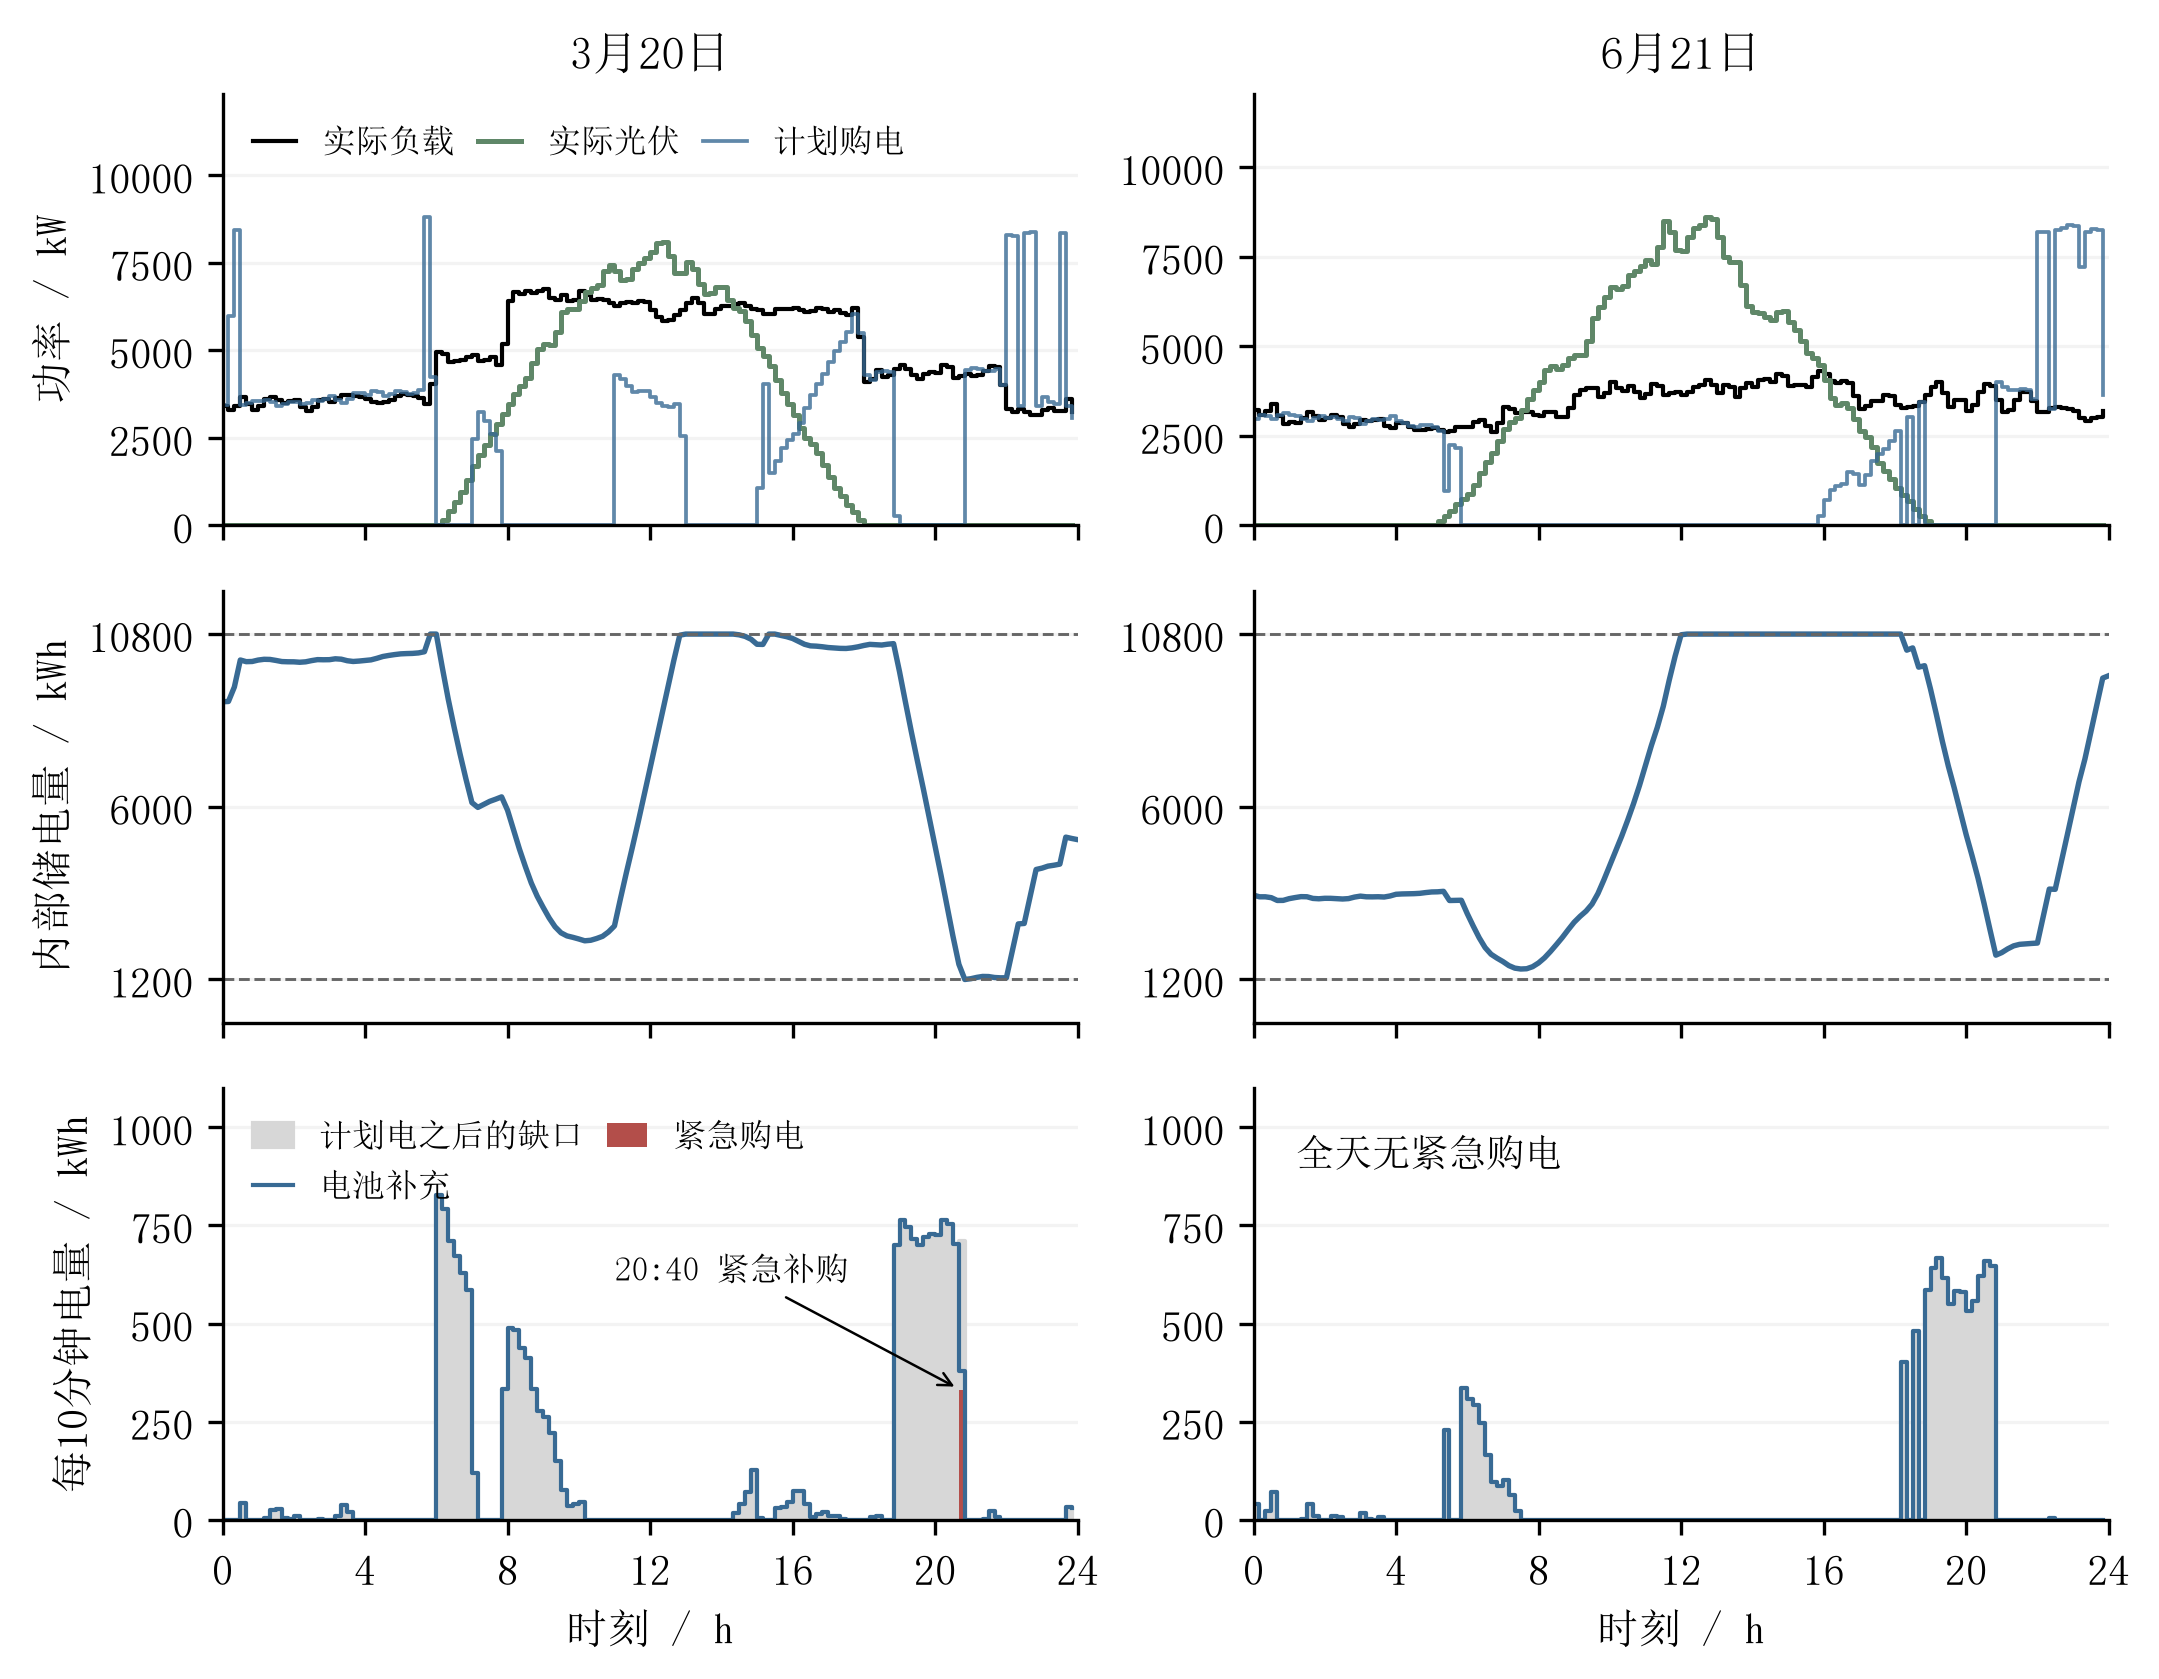
\includegraphics[width=\textwidth]{fig/specified_days.png}
    \caption{两个指定日期的供需、储电量与缺口补充情况}
    \label{fig:q2_specified_days}
\end{figure}

3月20日的大部分供需偏差均由电池吸收，但20:40时电池已接近最低储电量，放电后达到1200 kWh下限，因此剩余$329.52$ kWh只能通过紧急购电补足。

相比之下，6月21日白天有较多光伏可以用于充电，电池能够在后续时段持续补充负载缺口，因此全天没有发生紧急购电。

图\ref{fig:q2_specified_days}说明，是否需要紧急购电不能只比较全天总电量，还必须考虑\textbf{缺口出现的时刻、当时的储电量以及电池的放电能力}。


\subsection{灵敏度与风险分析}

图\ref{fig:q2_sensitivity}分别考察准备程度$\alpha$和时间衰减参数$\beta$对总费用的影响。

\begin{figure}[H]
    \centering
    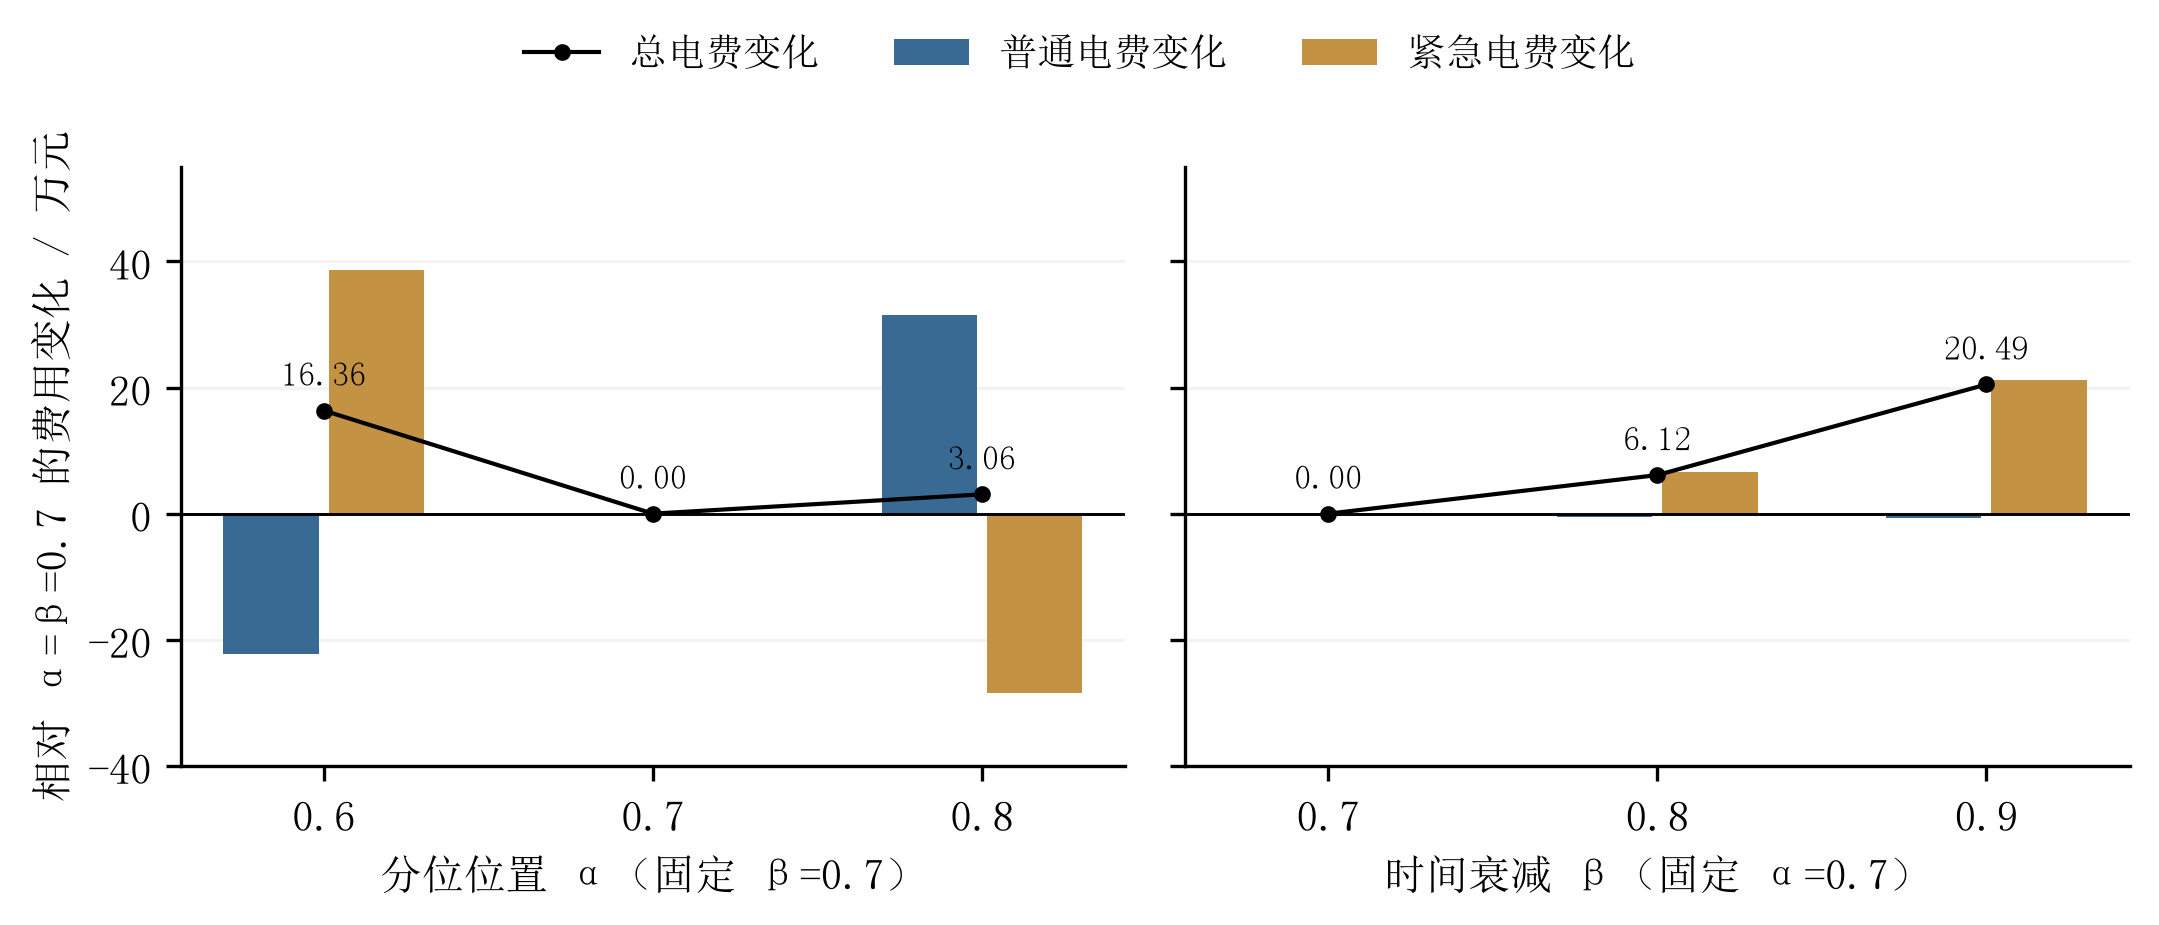
\includegraphics[width=0.95\textwidth]{fig/sensitivity.png}
    \caption{准备程度与近期权重对购电费用的影响}
    \label{fig:q2_sensitivity}
\end{figure}

当固定$\beta=0.7$时：

\begin{itemize}
    \item $\alpha=0.6$时，准备不足，总费用增加约$16.36$万元；
    \item $\alpha=0.8$时，虽然紧急购电减少，但普通购电增加更多，总费用仍增加约$3.06$万元。
\end{itemize}

当固定$\alpha=0.7$时，将$\beta$提高到0.8和0.9，总费用分别增加约$6.12$万元和$20.49$万元。

因此，\textbf{准备量并非越多越好}。准备不足会增加紧急购电，准备过多又会增加普通购电成本。在本文所测试的参数中，$\alpha=\beta=0.7$的费用较低，但这并不表示其为所有连续参数取值中的唯一最优解。

最终方案仍有部分日期发生紧急购电。这是因为储能设备的容量和放电功率均有限。储能能够缓冲预测误差，但不能完全消除实际供需变化带来的风险。